\documentclass[journal,12pt,twocolumn]{IEEEtran}

\usepackage{enumitem}
\usepackage{amsmath}
\usepackage{amssymb}
\usepackage{gensymb}
\usepackage{graphicx}
\usepackage{txfonts}         
\usepackage{listings}
\usepackage{lstautogobble}
\usepackage{mathtools}

\newcommand{\solution}{\noindent \textbf{Solution: }}
\providecommand{\pr}[1]{\ensuremath{\Pr\left(#1\right)}}
\providecommand{\brak}[1]{\ensuremath{\left(#1\right)}}
\providecommand{\cbrak}[1]{\ensuremath{\left\{#1\right\}}}
\providecommand{\sbrak}[1]{\ensuremath{\left[#1\right]}}
\providecommand{\mean}[1]{E\left[ #1 \right]}
\providecommand{\var}[1]{\mathrm{Var}\left[ #1 \right]}
\providecommand{\der}[1]{\mathrm{d} #1}

\let\StandardTheFigure\thefigure
\numberwithin{equation}{section}
\renewcommand{\thefigure}{\theenumi}
\renewcommand\thesection{\arabic{section}}

\lstset {
	frame=single, 
	breaklines=true,
	columns=fullflexible,
	autogobble=true
}             
                               
\title{Random Numbers }
\author{Ravula Karthik \\ \normalsize AI21BTECH11024 \\ \vspace*{20pt} \normalsize }


\begin{document}

	\maketitle
	
	\section{Uniform Random Numbers}
	Let $U$ be a uniform random variable between 0 and 1.
	\begin{enumerate}[label=\thesection.\arabic*,ref=\thesection.\theenumi]
	\item Generate $10^6$ samples of $U$ using a C program and save into a file called uni.dat

	\solution The c code for 1.1 can be obtained from
	\begin{lstlisting}
		wget https://github.com/karthik6281/AI1110-Assignments/blob/main/random_numbers/1/exrand.c
		wget https://github.com/karthik6281/AI1110-Assignments/blob/main/random_numbers/1/coeffs.h
	\end{lstlisting}
	Execute the following lines
	\begin{lstlisting}
		gcc exrand.c -lm
		./a.out
	\end{lstlisting}
	\item Load the uni.dat file into Python and plot the empirical CDF of $U$ using the samples in uni.dat. The CDF is defined as
	\begin{align}
		F_{U}(x) = \pr{U \le x}
	\end{align}

	\solution  The python code for 1.2 can be obtained from
	\begin{lstlisting}
		wget https://github.com/karthik6281/AI1110-Assignments/blob/main/random_numbers/1/cdf_plot.py
	\end{lstlisting}
	Execute the following lines
	\begin{lstlisting}
		python3 1_2.py
	\end{lstlisting}
	\begin{figure}
		\centering
		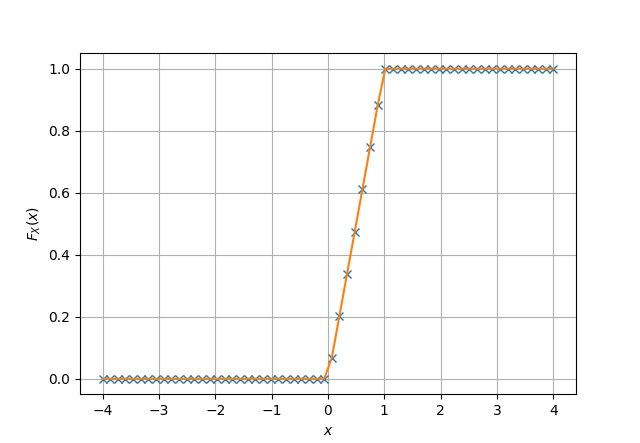
\includegraphics[width=\columnwidth]{./figs/cdf_plot.png}
		\caption{The CDF of $U$}
		\label{fig-1.2}
	\end{figure}
	
	\item Find a  theoretical expression for $F_{U}(x)$
	
	\solution The PDF of $U$ is given by
	\begin{align}
		p_{U}(x) = 
		\begin{cases}
			1 & x \in [0, 1] \\
			0 & \text{otherwise}
		\end{cases}
	\end{align}
	
	The CDF of $U$ is given by
	\begin{align}
		F_{U}(x) = \pr{U \le x} = \int_{-\infty}^x p_{U}(x) ~\mathrm{d}x
	\end{align}
	
	If $x<0$,
	\begin{align}
		\int_{-\infty}^x p_{U}(x) ~\mathrm{d}x = \int_{-\infty}^x 0 ~\mathrm{d}x = 0
	\end{align}
	
	If $x \in [0, 1]$,
	\begin{align}
		\int_{-\infty}^x p_{U}(x) ~\mathrm{d}x &= \int_{-\infty}^0 0 ~\mathrm{d}x + \int_0^x 1 ~\mathrm{d}x \\
		&= 0 + x \\
		&= x
	\end{align}
	
	If $x>1$,
	\begin{multline}
		\int_{-\infty}^x p_{U}(x) ~\mathrm{d}x \\= \int_{-\infty}^0 0 ~\mathrm{d}x + \int_0^1 1 ~\mathrm{d}x +  \int_1^x 0 ~\mathrm{d}x 
	\end{multline}
	\begin{align}
		\int_{-\infty}^x p_{U}(x) ~\mathrm{d}x &= 0 + 1 + 0 \\
		&= 1
	\end{align}
	
	Therefore, we obtain the CDF of $U$ as
	\begin{align}
		F_{U}(x) = 
		\begin{cases}
			0 & x < 0 \\
			x & 0 \le x \le 1 \\
			1 & x > 1
		\end{cases}
	\end{align}
	
	\item The mean of $U$ is defined as
	\begin{align}
		\mean{U} = \frac{1}{N}\sum_{i=1}^{N}U_i
	\end{align}
	and its variance as
	\begin{align}
		\var{U} = \mean{U- \mean{U}}^2 
	\end{align}
	Write a C program to  find the mean and variance of $U$
	
	\solution The c code for 1.4 can be obtained from
	\begin{lstlisting}
	wget https://github.com/karthik6281/AI1110-Assignments/blob/main/random_numbers/1/1_4.c
	wget https://github.com/karthik6281/AI1110-Assignments/blob/main/random_numbers/1/coeffs.h
	\end{lstlisting}
	Execute the following lines
	\begin{lstlisting}
		gcc 1_4.c -lm
		./a.out
	\end{lstlisting}
	\begin{align}
		\text{Mean} &= 0.500137 \\
		\text{Variance} &= 0.083251
	\end{align}
	
	\item Verify your result theoretically given that
	\begin{align}
		\mean{U^k} = \int_{-\infty}^{\infty}x^k \mathrm{d}F_{U}(x)
	\end{align}
		
	\solution 
		\begin{equation}
E\sbrak{U^k} = \int_{-\infty}^{\infty}x^kdF_{U}(x)
\end{equation}
\begin{align}
&dF_{U}(x)=dx\\
&\therefore E[U^k]=\int_{-\infty}^{\infty} x^k dx\\
&E[U]=\int_{0}^{1} x dx=\frac{1}{2}\\
&E[U^2]=\int_{0}^{1} x^2 dx=\frac{1}{3}\\
&\because P_{X}(x)=0 ,\forall x \in (1,\infty)\cap (-\infty,0)\\
&Var(X)=E[U^2]-(E[U])^2=\frac{1}{3}-\frac{1}{4}=\frac{1}{12}
\end{align}
	
	\section{Central Limit Theorem}

	\begin{enumerate}[label=\thesection.\arabic*,ref=\thesection.\theenumi]
	\item Generate $10^6$ samples of the random variable
	\begin{align}
		X = \sum_{i=1}^{12}U_i -6
	\end{align}

	using a C program, where $U_i, i = 1,2,\dots, 12$ are  a set of independent uniform random variables between 0 and 1 and save in a file called gau.dat
	
	\solution The c code for 2.1 can be obtained from
	\begin{lstlisting}
		wget https://github.com/karthik6281/AI1110-Assignments/blob/main/random_numbers/2/2_1.c
		wget https://github.com/karthik6281/AI1110-Assignments/blob/main/random_numbers/2/coeffs.h
	\end{lstlisting}
	Execute the following lines
	\begin{lstlisting}
		gcc 2_1.c -lm
		./a.out
	\end{lstlisting}
		
	\item Load gau.dat in Python and plot the empirical CDF of $X$ using the samples in gau.dat. What properties does a CDF have?

	\solution The python code for 2.2 can be obtained from
	\begin{lstlisting}
		wget https://github.com/karthik6281/AI1110-Assignments/blob/main/random_numbers/2/2_2.py
	\end{lstlisting}
	Execute the following lines
	\begin{lstlisting}
		python3 2_2.py
	\end{lstlisting}
	\begin{figure}
		\centering
		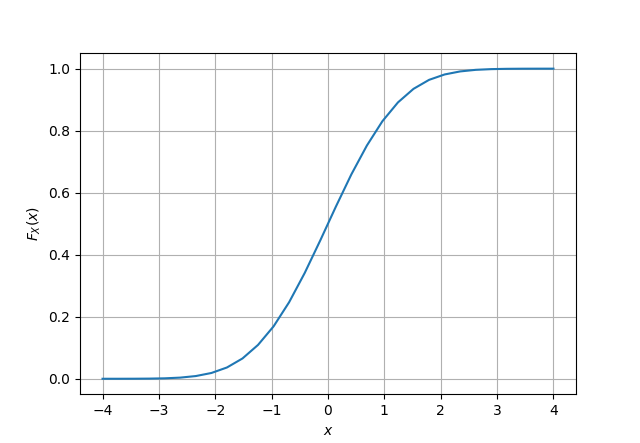
\includegraphics[width=\columnwidth]{./figs/2_2_fig.png}
		\caption{The CDF of $X$}
		\label{fig-2.2}
	\end{figure}
	
	\begin{itemize}
\item $\Phi(x)=P(Z \leq x)= \frac{1}{\sqrt{2 \pi}} \int_{-\infty}^{x}\exp\left\{-\frac{u^2}{2}\right\} du$
\item $\lim \limits_{x\rightarrow \infty} \Phi(x)=1, \hspace{5pt} \lim \limits_{x\rightarrow -\infty} \Phi(x)=0$
\item  $\Phi(0)=\frac{1}{2}$
\item  $\Phi(-x)=1-\Phi(x)$
\end{itemize}
	\item Load gau.dat in Python and plot the empirical PDF of $X$ using the samples in gau.dat. The PDF of $X$ is defined as
	\begin{align}
		p_{X}(x) = \frac{\der{}}{\der{x}}F_{X}(x)
	\end{align}
	What properties does the PDF have?
	
	\solution The python code for 2.3 can be obtained from
	\begin{lstlisting}
		wget https://github.com/karthik6281/AI1110-Assignments/blob/main/random_numbers/2/2_3.py
	\end{lstlisting}
	Execute the following lines
	\begin{lstlisting}
		python3 2.3.py
	\end{lstlisting}
	\begin{figure}
		\centering
		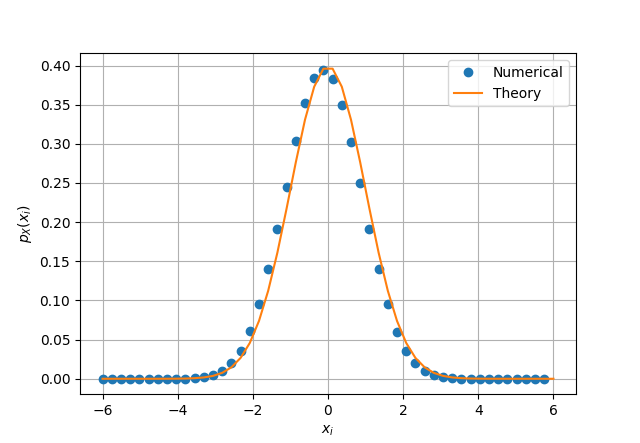
\includegraphics[width=\columnwidth]{./figs/2_3_fig.png}
		\caption{The PDF of $X$}
		\label{fig-2.3}
	\end{figure}
	
	Every PDF is bounded between $0$ and $1$ and
	\begin{align}
		\int_{-\infty}^{\infty} p_{X}(x) ~\mathrm{d}x = 1
	\end{align}
	
	In this case, the PDF is symmetric about $x = 0$ and graph is bell shaped
	
	\item Find the mean and variance of $X$ by writing a C program
	
	\solution the c code for 2.4 can be obtained from
	\begin{lstlisting}
		wget https://github.com/karthik6281/AI1110-Assignments/blob/main/random_numbers/2/2_4.c
		wget https://github.com/karthik6281/AI1110-Assignments/blob/main/random_numbers/2/coeffs.h
	\end{lstlisting}
	execute the following lines
	\begin{lstlisting}
		gcc 2_4.c -lm
		./a.out
	\end{lstlisting}
	\begin{align}
		\text{Mean} &= 0.000294 \\
		\text{Variance} &= 0.999561 
	\end{align}	
	
	\item Given that
	\begin{align}
		p_{X}(x) = \frac{1}{\sqrt{2\pi}}\exp\brak{-\frac{x^2}{2}}, -\infty < x < \infty,
	\end{align}
	repeat the above exercise theoretically
	
	\solution The mean of $X$ is given by
	\begin{align}
		\mean{X} &= \int_{-\infty}^{\infty} \frac{x}{\sqrt{2\pi}}\exp\brak{-\frac{x^2}{2}} \mathrm{d}x 
	\end{align}
	$\implies x e^{-\frac{-x^2}{2}} $
	\text{is a odd function}
	\begin{align}
		\therefore \mean{X} &= \int_{-\infty}^{\infty} g(x) \mathrm{d}x = 0
	\end{align}
	
	Now, 
	\begin{align}
		\mean{X^2} &= \int_{-\infty}^{\infty} \frac{x^2}{\sqrt{2\pi}}\exp\brak{-\frac{x^2}{2}} \mathrm{d}x \\
		&= 2 \int_{0}^{\infty} \frac{x^2}{\sqrt{2\pi}}\exp\brak{-\frac{x^2}{2}} \mathrm{d}x
	\end{align}
	$\implies \frac{x^2}{\sqrt{2\pi}}\exp\brak{-\frac{x^2}{2}}$ is an even function
	
	By integration by parts,
	\begin{align}
		\mean{X^2} = \sqrt{\frac{2}{\pi}}  \int_{0}^{\infty} x \cdot x \exp\brak{-\frac{x^2}{2}} \der{x} 
	\end{align}
	\begin{multline}
		= \sqrt{\frac{2}{\pi}} \brak{\left. x \int x \exp\brak{-\frac{x^2}{2}} \der{x}}\right|_0^{\infty} \\- \sqrt{\frac{2}{\pi}}  \int_{0}^{\infty} 1 \cdot \int x \exp\brak{-\frac{x^2}{2}} \der{x}
	\end{multline}
	
	Substitute $t = \frac{x^2}{2} \implies \der{t} = x\der{x}$
	\begin{align}
		\int x \exp\brak{-\frac{x^2}{2}} \der{x} &= \int \exp(-t) \der{t} \\
		&= - \exp(-t) \\
		&= - \exp\brak{-\frac{x^2}{2}}
	\end{align}
	
	\begin{align}
		&\int_0^{\infty} - \exp\brak{-\frac{x^2}{2}} \der{x} \\
		\xleftrightarrow{x = t\sqrt{2}} &\int_0^{\infty} -\exp(-t^2) \der{t}\sqrt{2} \\
		&= -{\sqrt{2}} \int_0^{\infty} \exp(-t^2) \der{t} \\
		&= - \sqrt{\frac{\pi}{2}}
	\end{align}
	
	Therefore,
	\begin{align}
		\mean{X^2} &= 0 - \sqrt{\frac{2}{\pi}} \brak{- \sqrt{\frac{\pi}{2}}} \\
		&= 1 \\
		\therefore \var{X} &= \mean{X^2} - \brak{\mean{X}}^2 \\
		&= 1 - 0 \\
		&= 1
	\end{align}
	\end{enumerate}
	
	\section{From Uniform to Other}
	\begin{enumerate}[label=\thesection.\arabic*,ref=\thesection.\theenumi]
	\item Generate samples of 
	\begin{align}
		V = -2\ln\brak{1-U}
	\end{align}
	and plot its CDF
	\end{enumerate}
	\solution The c code for 3.1 can be obtained from
	\begin{lstlisting}
		wget https://github.com/karthik6281/AI1110-Assignments/blob/main/random_numbers/3/3_1.c
	\end{lstlisting}
	Execute the following lines
	\begin{lstlisting}
		gcc 3.1.c -lm
		./a.out
	\end{lstlisting}
	The python code for cdf can be obtained from
	\begin{lstlisting}
		wget https://github.com/karthik6281/AI1110-Assignments/blob/main/random_numbers/3/3_1.py
	\end{lstlisting}
	execute the following lines
	\begin{lstlisting}
		python3 3_1.py
	\end{lstlisting}
	\begin{figure}
		\centering
		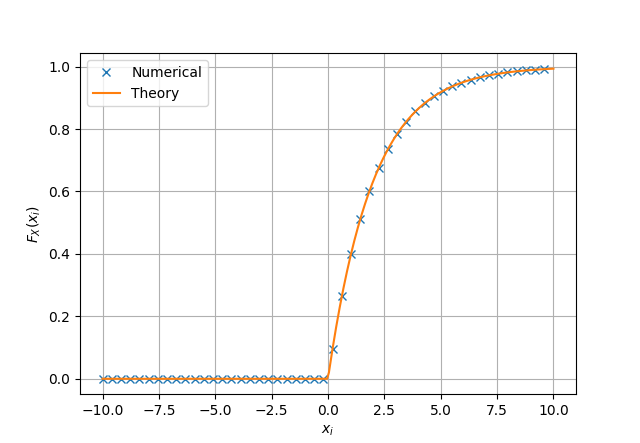
\includegraphics[width=\columnwidth]{./figs/3_1_cdf.png}
		\caption{The CDF of $V$}
		\label{fig-3.1}
	\end{figure}	
	
	\item Find a theoretical expression for $F_V(x)$
	
	\solution \begin{align}
 &F_{V}(x)=P(V \leq x)\\
 &=P(-2 ln(1-U) \leq x)\\
 &=P(1-e^{\frac{-x}{2}} \geq U)\\
 &P(U<x)=\int_{0}^{x} dx=x\\
 &\therefore P(1-e^{\frac{-x}{2}} \geq U)=1-e^{\frac{-x}{2}}, \forall x\geq 0 \\ 
 \nonumber
 \end{align}
	
	\section{Triangular Distribution}
	\begin{enumerate}[label=\thesection.\arabic*,ref=\thesection.\theenumi]
	\item Generate 
	\begin{align}
		T = U_1+U_2
	\end{align}
	\solution The c code for 4.1 can be obtained from
	\begin{lstlisting}
		wget https://github.com/karthik6281/AI1110-Assignments/blob/main/random_numbers/4/4_1.c
	\end{lstlisting}
	execute the following lines
	\begin{lstlisting}
		gcc 4_1.c -lm
		./a.out
	\end{lstlisting}
	
	\item Find the CDF of $T$
	
	\solution The CDF of $T$ is given by
	\begin{align}
		F_T(t) = \pr{T \le t} = \pr{U_1 + U_2 \le t}	
	\end{align}		
	Since $U_1, U_2 \in [0,1] \implies U_1 + U_2 \in [0,2]$
	Therefore, if $t \ge 2$, then $U_1 + U_2 \le t$ is always true and if $t < 0$, then $U_1 + U_2 \le t$ is always false.
	
	Now, fix the value of $U_1$ to be some $x$
	\begin{align}
		x + U_2 \le t \implies U_2 \le t - x
	\end{align}
	
	If $0 \le t \le 1$, then $x$ can take all values in $[0,t]$
	\begin{align}
		F_T(t)	&= \int_0^t \pr{U_2 \le t - x} p_{U_1}(x) \der{x} \\
		&= \int_0^t F_{U_2}(t-x) p_{U_1}(x) \der{x}
	\end{align}
	\begin{align}
		0 \le x \le t &\implies 0 \le t - x \le t \le 1 \\
		&\implies F_{U_2}(t-x) = t - x
	\end{align}
	\begin{align}
		F_T(t) &= \int_0^t (t-x) \cdot 1 \cdot \der{x} \\
		&= \left. tx - \frac{x^2}{2} \right|_0^t \\
		&= \frac{t^2}{2}
	\end{align}
	
	If $1 < t < 2$, $x$ can only take values in $[0,1]$ as $U_1 \le 1$
	\begin{align}
		F_T(t)	&= \int_0^1 F_{U_2}(t-x) \cdot 1 \cdot \der{x} 
	\end{align}
	\begin{align}
		0 \le x \le t - 1 &\implies 1 \le t - x \le t \\
		t - 1 \le x \le 1 &\implies 0 < t - 1 \le t - x \le 1
	\end{align}
	\begin{align}
		F_T(t) &= \int_0^{t-1} 1 \der{x} + \int_{t-1}^1 (t-x)\der{x} \\
		&= t - 1 + t(1 - (t - 1)) - \frac{1}{2} + \frac{(t-1)^2}{2} \\
		&= t - 1 + 2t - t^2 -\frac{1}{2} + \frac{t^2}{2} + \frac{1}{2} - t \\ 
		&= -\frac{t^2}{2} + 2t - 1
	\end{align}
	
	Therefore,
	\begin{align}
		F_T(t) = 
		\begin{cases}
		0 & t < 0 \\
		\dfrac{t^2}{2} & 0 \le t \le 1 \\
		 2t -\dfrac{t^2}{2} - 1 & 1 < t < 2 \\
		1 & t \ge 2
		\end{cases}
	\end{align}
	
		
	
	\item Find the PDF of $T$
	
	\solution The PDF of $T$ is given by
	\begin{align}
		p_T(t) &= \frac{d(F_{T}(t))}{dt} \\
		\therefore p_T(t) &=
		\begin{cases}
			0 & t < 0 \\
			t & 0 \le t \le 1 \\
			2 - t & 1 < t < 2 \\
			0 & t \ge 2
		\end{cases}
	\end{align}
	
	\item Find the theoretical expressions for the PDF and CDF of $T$
	
	\solution 
\begin{align}
P_{T}(t)=
\begin{cases}
0 & t<0\\
t & 0\leq t \leq 1\\
2-t  & 0< t \leq 2\\
0 & t>2 
\end{cases} 
\\   
F_{T}(t)=
\begin{cases}
0 & t<0\\
\frac{t^2}{2} & 0\leq t \leq 1\\
2t -\dfrac{t^2}{2} - 1  & 1< t \leq 2\\
1 & t>2
\end{cases}
\end{align}
	\item Verify your results through a plot
	
	\solution The codes that plots cdf and pdf can be obtained from
	\begin{lstlisting}
		wget https://github.com/karthik6281/AI1110-Assignments/blob/main/random_numbers/4/4_cdf.py
		wget https://github.com/Ankit-Saha-2003/AI1110/raw/main/Random-Numbers/codes/4.3.py
	\end{lstlisting}
	Execute the following lines
	\begin{lstlisting}
		python3 4_cdf.py
		python3 4_pdf.py
	\end{lstlisting}
	
	
	\end{enumerate}
	
	\begin{figure}
		\centering
		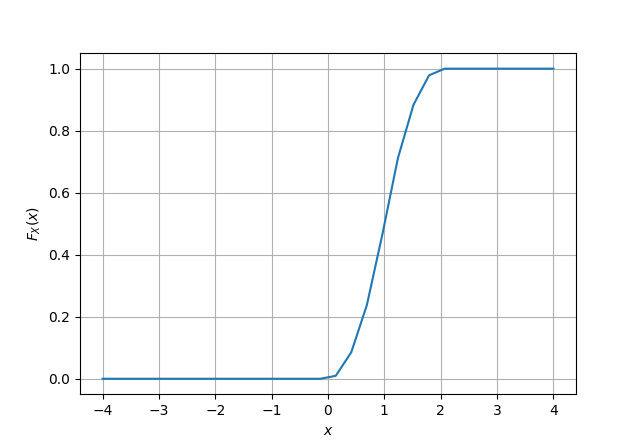
\includegraphics[width=\columnwidth]{./figs/4_cdf.png}
		\caption{The CDF of $T$}
	\end{figure}
	
	\begin{figure}
		\centering
		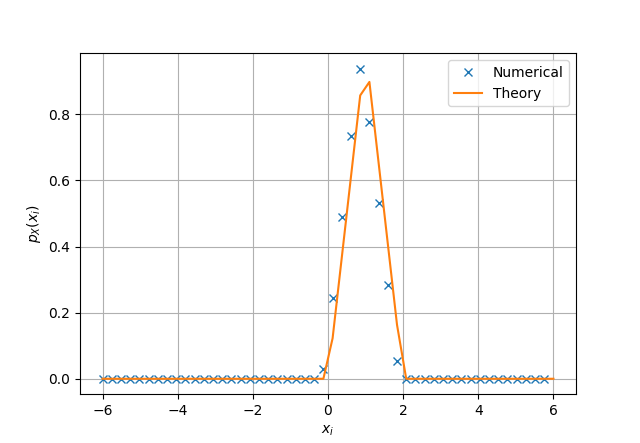
\includegraphics[width=\columnwidth]{./figs/4_pdf.png}
		\caption{The PDF of $T$}
	\end{figure}		
	
\end{document}
